\chapter{Theoretische Grundlagen}
In diesem Kapitel werden die zentralen theoretischen Grundlagen vermittelt, die für das Verständnis der Arbeit und die spätere Umsetzung notwendig sind.
Es werden sowohl technische Aspekte von WordPress und der Plugin-Entwicklung als auch die Prinzipien des Gutenberg-Editors betrachtet.
Ergänzend werden konzeptionelle Überlegungen zu Gamification und gesellschaftlich relevanten Plattformen diskutiert, um den fachlichen Rahmen der Arbeit abzustecken.

\section{WordPress als Content-Management-System}
WordPress ist ein freies, unter der \gls{gnu} \gls{gpl} v2 lizenziertes Content-Management-System und mit einem Marktanteil von 61,1\% das weltweit am häufigsten verwendete \gls{cms}~\cite{statista2025cms}.
Die Plattform zeichnet sich durch seine Flexibilität, Erweiterbarkeit und Bedienbarkeit aus, was WordPress zu einer Lösung für simple Webseiten und Blogs bis hin zu komplexe Web-Applikationen macht~\cite{patel2019review}.
Die technische Struktur verfolgt ein modulares Paradigma, das eine klare Trennung zwischen Kernfunktionen, Design und Erweiterungen ermöglicht:
\begin{itemize}

 \item Themes: Kontrollieren die Präsentationslogik und das Design der Webseite

 \item Plugins: Erweitern die Funktionalität

 \item Core System: Stellt die grundlegenden Funktionen des \gls{cms} bereit

\end{itemize}
Technisch gesehen besteht WordPress aus einer \gls{php}-basierten Architektur in Verbindung mit der persistenten Speicherlösung \gls{mysql} als relationale Datenbank.
Durch diese weit verbreiteten Technologien ist WordPress mit den meisten gängigen Hosting-Umgebungen kompatibel.
Grundlage hierfür ist ein Webserver, welcher \gls{php} und \gls{mysql} unterstützt.
Offiziell ist Apache oder Nginx empfohlen~\cite{wordpress2024requirements}.

Darüber hinaus bietet WordPress eine \gls{rest}-\gls{api} mit der eine entkoppelte Inhaltsverwaltung möglich ist und Inhalte über das \gls{http}-Protokoll in verschiedene Anwendungen und Plattformen integriert werden können.
\newpage
\textbf{WordPress Coding Standards}

WordPress Coding Standards dienen als Richtlinien und Best Practises für Entwickler die an WordPress Projekten arbeiten.
Diese Standards haben sich in der Wordpress Community etabliert und ermöglichen eine konsistente Codestruktur.
Ziel ist es, die Codequalität so zu gestalten, dass Wartung und kollaborative Weiterentwicklung erleichtert werden.
Für die Ausarbeitung der Weiterentwicklung von Charigame sollen die offiziellen Wordpress Coding Standards beachtet und umgesetzt werden~\cite{wordpress2024codingstandards}.


\section{Plugin-Entwicklung mit WordPress}

Die offizielle WordPress-Definition besagt: \glqq \gls{plugin}s sind Codepakete, die die Kernfunktionalität von WordPress erweitern.
WordPress-\gls{plugin}s bestehen aus \gls{php}-Code und können weitere Assets wie Bilder,
\gls{css} und JavaScript enthalten\grqq{} \cite{wordpress2024plugin} (eigene Übersetzung).
\\ \\
Für die Entwicklung solcher \gls{plugin}s ist grundlegend ein tiefergehendes Verständnis des WordPress-\gls{cms} vorausgesetzt.
Die Grundlagen sowie weiterführende Themengebiete sollen im Folgenden ermittelt werden.



\subsection{Grundlagen der Plugin-Architektur}

Die Entwicklung von \gls{plugin}s in WordPress setzt ein Basiswissen der Dateistruktur und des internen Aufbaus des Content-Management-Systems voraus.
Insbesondere ist es erforderlich, die \gls{plugin}-bezogenen Dateien korrekt zu strukturieren und im entsprechenden Verzeichnis innerhalb der WordPress-Installation zu platzieren.\\\\
\gls{plugin}s werden standardmäßig im Verzeichnis \texttt{wp-content/plugins} abgelegt.
Jeder \gls{plugin}-Ordner enthält dabei alle notwendigen Dateien zur Funktionalität des jeweiligen Moduls.\\\\
Im folgenden Schaubild ist eine typische, nicht modifizierte Verzeichnisstruktur einer WordPress-Installation dargestellt.
Diese dient als Ausgangspunkt für die Entwicklung und Integration von \gls{plugin}s:

\begin{figure}[tbh]
 \centering
 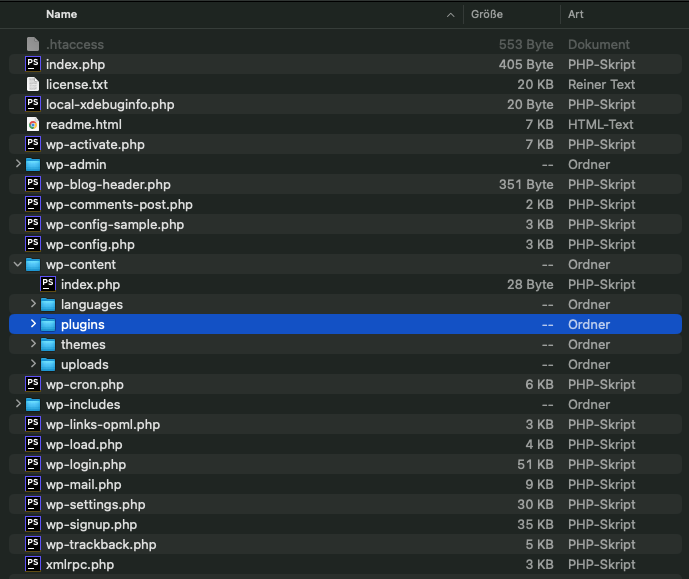
\includegraphics[width=0.88\textwidth]{wordpress_ordner_aufbau}
 \caption{Unveränderte WordPress-Verzeichnisstruktur der Version 6.8.2 (eigene Darstellung)}
 \label{fig:wordpress-verzeichnis}
\end{figure}
\newpage
Abbildung~\ref{fig:wordpress-verzeichnis} visualisiert, dass sich im wp-content Ordner bereits initial in der Standardkonfiguration von Wordpress das Verzeichnis plugins befindet.
Der plugins Ordner ist die zentrale Destination für alle im WordPress System erstellten Erweiterungen.
Die nachfolgende Untersuchung berücksichtigt weitere Bestandteile von WordPress-\gls{plugin}s, die fortlaufend detailliert beschrieben werden.
\\\\
\textbf{Aufbau, Plugin-Header und Metadateien}

Für die Entwicklung von WordPress-\gls{plugin}s empfehlen die offiziellen WordPress Developer Resources eine klare und strukturierte Ordnerorganisation. \cite{wordpress2024BestPractices}
Als empfohlen wird folgende grundlegende Verzeichnisstruktur vorgeschlagen (vgl. Abbildung~\ref{fig:wp-plugin-structure}):
\\\\\\
\begin{figure}[H]
    \centering
    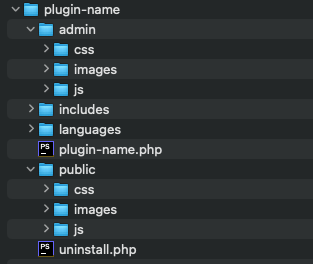
\includegraphics[width=0.4\textwidth]{images/wp_plugin_structure}
    \caption{Empfohlene Plugin Ordnerstruktur (eigene Darstellung angelehnt an Wordpress Developer Resources \cite{wordpress2024FolderStructure})}
    \label{fig:wp-plugin-structure}
\end{figure}

Die Datei plugin-name.php stellt im gezeigten Beispielaufbau die zentrale Plugindatei dar.
In dieser Datei muss eine von WordPress vorgegebene Headerstruktur enthalten sein, damit das System die Datei als Plugin erkennt und korrekt lädt.
Das minimale erforderliche Header-Format ist dabei wie in Abbildung~\ref{fig:wp-plugin-min} definiert:

\begin{figure}[H]
    \centering
    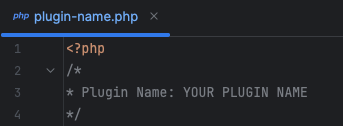
\includegraphics[width=0.4\textwidth]{images/wp_plugin_min}
    \caption{Minimaler Plugin-Header in WordPress (eigene Darstellung angelehnt an Wordpress Developer Resources \cite{wordpress2024HeaderRequirement})}
    \label{fig:wp-plugin-min}
\end{figure}

Darüber hinaus können weitere optionale Felder definiert werden wie:
Author URI für die Website des Plugin-Entwicklers, Text Domain
zur Internationalisierung und Domain Path für den Pfad zu Sprachdateien.
Alle möglichen Felder werden in der folgenden Tabelle aufgeführt:
\renewcommand{\arraystretch}{1.3}

\begin{longtable}{>{\bfseries}p{4cm} p{10cm}}
 \caption{Übersicht der Plugin-Header-Felder in WordPress nach \cite{wordpress2024HeaderRequirement}} \\
 \hline
 Feldname & Beschreibung \\
 \hline
 \endfirsthead

 \multicolumn{2}{l}{\textit{Fortsetzung von vorheriger Seite}} \\
 \hline
 Feldname & Beschreibung \\
 \hline
 \endhead

 \hline
 \multicolumn{2}{r}{\textit{Fortsetzung auf nächster Seite}} \\
 \endfoot

 \hline
 \endlastfoot

 Plugin Name (erforderlich) & Der Name des Plugins, wie er in der Plugin-Übersicht im WordPress-Adminbereich angezeigt wird. \\
 Plugin \gls{uri} & Eine eindeutige \gls{url} zur Startseite des Plugins, idealerweise auf der eigenen Website. WordPress.org-URLs sind hier nicht erlaubt. \\
 Description & Eine kurze Beschreibung des Plugins (max. 140 Zeichen), wie sie im WordPress-Adminbereich angezeigt wird. \\
 Version & Die aktuelle Versionsnummer des Plugins, z.\,B. \texttt{1.0} oder \texttt{1.0.3}. \\
 Requires at least & Die minimale WordPress-Version, mit der das Plugin kompatibel ist. \\
 Requires PHP & Die minimale benötigte PHP-Version für das Plugin. \\
 Author & Der Name des Autors oder der Autoren des Plugins. Mehrere Autoren können durch Kommata getrennt angegeben werden. \\
 Author URI & Die Website des Autors oder ein öffentliches Profil, z.\,B. auf WordPress.org. \\
 License & Die Kurzbezeichnung der Lizenz, unter der das Plugin veröffentlicht wird (z.\,B. \texttt{GPLv2}). \\
 License URI & Ein Link zum vollständigen Lizenztext (z.\,B. \url{https://www.gnu.org/licenses/gpl-2.0.html}). \\
 Text Domain & Die Textdomain für die Internationalisierung des Plugins, erforderlich für Übersetzungen mit \texttt{gettext}. \\
 Domain Path & Das Verzeichnis, in dem WordPress die Übersetzungsdateien findet (z.\,B. \texttt{/languages}). \\
 Network & Gibt an, ob das Plugin netzwerkweit (Multisite) aktiviert werden kann. Nur \texttt{true} ist erlaubt, andernfalls Feld weglassen. \\
 Update URI & Eine eindeutige \gls{uri} zur Updatequelle, um versehentliche Überschreibungen durch gleichnamige Plugins im WordPress.org-Verzeichnis zu vermeiden. \\
 Requires Plugins & Eine durch Kommas getrennte Liste von Plugin-Slugs aus dem WordPress.org-Verzeichnis, die als Abhängigkeit benötigt werden. Kommas innerhalb der Slugs sind nicht erlaubt. \\
\end{longtable}

\newpage
\textbf{Hooks: Action und Filter}

Es gibt eine Kardinalregel in der Wordpress Entwicklung die besagt: Don’t touch WordPress core \cite{wordpress2024Intro}. %TODO: https://developer.wordpress.org/plugins/intro/ maybe verlinken?
Damit Anpassungen an bestehende Funktionalitäten möglich sind gibt es Hooks und Filter.
Hooks erlauben es an spezifischen Stellen einzugreifen, um das Verhalten von WordPress zu ändern ohne dabei die Kern-Dateien bearbeiten zu müssen.
Allgemein gibt es zwei Arten von hooks in WordPress: Actions und Filter.
Mit Actions können Funktionen hinzugefügt oder geändert werden.
Filter wiederum ändern Inhalte, während diese geladen und dem Website-Nutzer angezeigt werden.
Hooks sind nicht nur für die Plugin-Entwicklung gedacht, sondern werden ebenfalls häufig verwendet, um Standardfunktionen durch den WordPress-Kern selbst bereitzustellen.

Zu den zentralen Hooks im Kontext von WordPress-Plugins gehören insbesondere \texttt{register\_activation\_hook()}, \texttt{register\_deactivation\_hook()} sowie \\ \texttt{register\_uninstall\_hook()}~\cite{wordpress2024ActionsHooks}.

\begin{itemize}
 \item \textbf{register\_activation\_hook()}: Dieser Hook wird ausgeführt, wenn das Plugin im WordPress-Backend aktiviert wird. Dies wird oftmals verwendet um Funktionen zwecks Einrichtung des Plugins bereitzustellen.
 \item \textbf{register\_deactivation\_hook()}: Der Deaktivierungs-Hook wird ausgeführt, wenn das Plugin deaktiviert wird. Diese Funktion ermöglicht es die vom Plugin temporär gespeicherten Daten und Einträge zu entfernen.
 \item \textbf{register\_uninstall\_hook()}: Die Ausführung findet statt, wenn das Plugin aus dem Backend gelöscht wird. Die Verwendung zielt häufig darauf ab alle vom Plugin erstellen Optionen oder Datenbanktabellen restlos zu löschen.
\end{itemize}

%Plugin-Struktur und -Organisation

%Das WordPress Hook-System verstehen

%Plugin-Header und Metadaten

%Aktivierung und Deaktivierung von Plugins

%Plugin-Hauptdatei und Ordnerstruktur

\subsection{Best Practises in der Plugin-Programmierung}
Die WordPress Developer Resources geben dem Entwickler einige Best Practises vor, welche helfen den Code zu organisieren.
Ferner wird durch die Hinweise sichergestellt, dass der Code verlässlich mit dem WordPress Kern und anderen Plugins funktioniert.
Nachfolgend sollen zentrale Best Practises aufgeführt werden, welche im Verlauf der Arbeit mit in der Konzeption berücksichtigt werden.
\\
\\\\
\textbf{Vermeiden von Namenskonflikten}

Namenskollisionen können durch die gleiche Benennung von Variablen, Funktionen oder Klassen zustandekommen.
Um einen solchen Namenskonflikt zu vermeiden wird es empfohlen einen globalen Namenspace zu definieren.
Dieser Namespace ermöglicht das Überschreiben von anderen Variablen, Funktionen und Plugins.
Innerhalb von Funktionen und Klassen definierte Variablen, sind hiervon nicht betroffen~\cite{wordpress2024Naming}.
\\
\\
\\\\
\textbf{Voranstellen eines Prefix}

Unter Zuhilfenahme eines Prefix können potenzielle Konflikte im Hinblick auf Aufrufe und Ausführungen mit anderen Plugins verhindert werden.
Das Handbuch empfiehlt hierzu ein einzigartiges Wort, welches vor verschiedene Deklarationen vorangestellt wird~\cite{wordpress2024ProceduralCodingMethod}.
Auf das ChariGame gemünzte Projekt könnte dies dann wie folgt aussehen:
\begin{itemize}
 \item function charigame\_save\_post();
 \item define ('CHARIGAME\_LICENSE', true);
 \item class CHARIGAME\_Admin{}
 \item namespace ChariGame;
 \item update\_option('charigame\_settings', \$settings)
\end{itemize}
\vspace{1em}
\textbf{Prüfung vorhandener Implementierungen}\\\\
Damit der Code robust und weniger fehleranfällig ist, gilt es in Anbetracht der Best Practises auf bestehende Implementationen von Programmierelementen zu prüfen \cite{wordpress2024CheckExisting}.
Dies geschieht unter Zuhilfenahme der folgenden von \gls{php} zur Verfügung gestellten Funktionen:
\begin{itemize}
 \item Variablen: isset()
 \item Function\_exists() %NICHT BENÖTIGT IN EIGENEM NAMESPACE
 \item Classes class\_exists()
 \item Constants defined()
\end{itemize}
\vspace{1em}
\textbf{Architekturmuster}\\\\
Die WordPress Developer Resources geben eine Hand voll mögliche Architekturmuster vor.
Diese können grob in drei Variationen kategorisiert werden:
\begin{itemize}
 \item Einzelne Plugin-Datei, die Funktionen enthält
 \item Einzelne Plugin-Datei, die eine Klasse, ein instanziiertes Objekt und optionale Funktionen enthält
 \item Eine Haupt-Plugin-Datei, sowie eine oder mehrere Klassendateien
\end{itemize}

Je nachdem welchen Umfang das Plugin anstrebt, gilt es die passende Lösung des Architekturmusters zu wählen.
Eine einzelne Plugin-Datei, die Funktionen enthält, stellt eine solide Basis für ein kleines Plugin zur Verfügung.
Die Variante eine Haupt-Plugin-Datei zu erstellen und mehrere Klassendateien aufzubauen bietet sich eher für Plugins mit einer größeren Codebasis an.

\subsection{Plugin Security und Privacy}
Ein essenzieller Aspekt bei der Programmierung von WordPress Plugins ist die Plugin Security und Privacy.
Damit die Sicherheit von Eingaben gegeben ist, werden Methoden wie Validating, Sanatizing und Escaping genutzt.
\\\\
\textbf{Validating}

\begin{quote}
 Das Validierung von Eingaben ist der Prozess, bei dem Daten anhand eines vordefinierten Musters (oder mehrerer Muster) mit einem eindeutigen Ergebnis getestet werden: gültig oder ungültig.
 Die Validierung ist im Vergleich zur Bereinigung ein spezifischerer Ansatz, aber beide haben ihre Berechtigung.
 \\[0.5em]
 \emph{(eigene Übersetzung nach \cite{wordpress2024plugin_validation})}
\end{quote}

Es werden auch seitens der WordPress Developer Ressourcen einfache Validierungsbeispiele genannt \cite{wordpress2024plugin_validation}:
\begin{itemize}
\item Überprüfung, ob Pflichtfelder ausgefüllt wurden
\item Überprüfung, ob eine eingegebene Telefonnummer nur Zahlen und Satzzeichen enthält
\item Überprüfung, ob eine eingegebene Zeichenfolge eine von fünf gültigen Optionen ist
\item Überprüfung, ob ein Mengenfeld größer als 0 ist
\end{itemize}
Die Validierung selbst wird in verschiedene Philosophien gegliedert, die nun kurz exemplarisch aufgefasst werden:
\begin{table}[h]
 \centering
 \renewcommand{\arraystretch}{1.3}
 \begin{tabular}{|p{3cm}|p{5cm}|p{6cm}|}
  \hline
  \textbf{Philosophie} & \textbf{Beschreibung} & \textbf{Beispiel Anwendung} \\
  \hline
  Safelist \newline (Allowlist)
  & Nur Werte aus einer vordefinierten Liste erlauben. Alles andere wird abgelehnt.
  & Dropdown-Auswahl für Sortieroptionen (z.\,B. ``date``, ``author``). Nur erlaubte Keys werden akzeptiert. \\
  \hline
  Blocklist \newline (Denylist)
  & Bestimmte bekannte, unerwünschte Werte verbieten. Unsicher, da neue unerlaubte Werte nicht erfasst werden.
  & Sperren von bekannten schädlichen Dateiendungen (z.\,B. ``.exe``, ``.bat``). \\
  \hline
  Format Detection
  & Prüfen, ob Eingabe einem bestimmten Muster entspricht.
  & Postleitzahl-Validierung mit Regex, E-Mail-Prüfung mit \texttt{is\_email()}, nur Ziffern mit \texttt{ctype\_digit()}. \\
  \hline
  Format Correction (Sanitization)
  & Eingaben akzeptieren, aber in ein sicheres Format umwandeln.
  & Benutzername mit  \newline \texttt{sanitize\_title()}, Typ-Cast von String zu Integer \texttt{(int)\$input}. \\
  \hline
 \end{tabular}
 \caption{Übersicht Validierungs-Philosophien mit Beispielen (eigene Darstellung)}
\end{table}

\newpage
Wenn keine Validierung möglich ist, bedienen sich WordPress Entwickler der Möglichkeit des Sanatizing und Escaping von Werten.
\\\\
\textbf{Sanitizing}

\begin{quote}
 Die Bereinigung von Eingaben ist der Prozess der Sicherung/Bereinigung/Filterung von Eingabedaten.
 Die Validierung ist der Bereinigung vorzuziehen, da sie spezifischer ist.
 Wenn jedoch eine „spezifischere“ Lösung nicht möglich ist, ist die Bereinigung die nächstbeste Option.
 \\[0.5em]
 \emph{(eigene Übersetzung nach \cite{wordpress2024plugin_sanitizing})}
\end{quote}


Bevor also Daten, die von Nutzenden stammen, in der Datenbank abgelegt oder weiterverarbeitet werden,
sollten sie bereinigt werden.
Damit werden Sicherheitslücken als auch ungewollte Inhalte zu vermieden.
Dafür stellt WordPress verschiedene Funktionen bereit, die sicherstellen, dass Eingaben ausschließlich
die vorgesehenen Zeichen oder Strukturen enthalten.
Ein häufig genutztes Beispiel ist die Verwendung von \texttt{sanitize\_text\_field()} für Freitextfelder.
Nachfolgend werden die seitens WordPress bereitgestellten Funktionen erläutert:

\begin{table}[h]
 \centering
 \begin{tabular}{|l|p{8cm}|}
  \hline
  \textbf{Funktion} & \textbf{Beschreibung} \\
  \hline
  \texttt{sanitize\_text\_field()} & Entfernt Tags, ungültige UTF-8-Zeichen, \newline Zeilenumbrüche, Tabs und überflüssige Leerzeichen. \\
  \hline
  \texttt{sanitize\_email()} & Validiert und bereinigt eine E-Mail-Adresse. \\
  \hline
  \texttt{sanitize\_file\_name()} & Entfernt unerlaubte Zeichen aus Dateinamen. \\
  \hline
  \texttt{sanitize\_hex\_color()} & Prüft und bereinigt Hex-Farbwerte (\#RRGGBB). \\
  \hline
  \texttt{sanitize\_html\_class()} & Bereinigt Klassennamen für \gls{html}-Attribute.                                                    \\
  \hline
  \texttt{sanitize\_key()} & Bereinigt Array-Keys oder Optionsnamen. \\
  \hline
  \texttt{sanitize\_option()} & Bereinigt Optionswerte in der Datenbank. \\
  \hline
  \texttt{sanitize\_title()} & Macht einen String zu einem URL-freundlichen Titel. \\
  \hline
  \texttt{sanitize\_user()} & Bereinigt Benutzernamen. \\
  \hline
  \texttt{wp\_kses()} & Filtert HTML nach erlaubten Tags/Attributen. \\
  \hline
  \texttt{wp\_kses\_post()} & Wie \texttt{wp\_kses()}, aber mit Standardregeln für Posts. \\
  \hline
 \end{tabular}
 \caption{Auswahl wichtiger WordPress-Sanitization-Funktionen \\(eigene Darstellung)}
\end{table}

\newpage

\textbf{Escaping}\\\\
Escaping transformiert Ausgabedaten so, dass kritische Zeichen (z.\,B. \grqq{}<\grqq{} wird zu \grqq{}\&lt;\grqq{}) nicht mehr als Code interpretiert werden. Dies verhindert \gls{xss}-Angriffe.\\\\
Das Prinzip lautet: Daten unverändert speichern, erst bei der Ausgabe escapen.
WordPress bietet kontextspezifische Funktionen wie \texttt{esc\_html()}, \texttt{esc\_attr()}, \texttt{esc\_url()} und \texttt{esc\_js()}~\cite{wordpress2024escapingfunc}.
Die richtige Funktionswahl je nach Ausgabekontext ist entscheidend für die Sicherheit.
Genau wie beim Sanatizing bietet WordPress hier ein Set an Funktionen, welche speziell für das Escaping genutzt werden.

\begin{table}[H]
 \centering
 \begin{tabular}{|l|p{9cm}|}
  \hline
  \textbf{Funktion} & \textbf{Anwendungsfall / Beschreibung} \\
  \hline
  \texttt{esc\_html()}      & Escaped Text für den Einsatz innerhalb von \gls{html}-Elementen. Entfernt sämtliches HTML. \\
  \hline
  \texttt{esc\_attr()} & Für Werte innerhalb von HTML-Attributen, z.\,B. \texttt{<input value=\grqq{}...\grqq{}>}. \\
  \hline
  \texttt{esc\_url()}       & Für \gls{url}s in \texttt{src} oder \texttt{href}-Attributen. \\
  \hline
  \texttt{esc\_url\_raw()} & Roh-URL-Escaping für Speicherung in der Datenbank oder nicht-encodierte Weitergabe. \\
  \hline
  \texttt{esc\_js()} & Für Inline-JavaScript oder Übergabe von Variablen in Skripte. \\
  \hline
  \texttt{esc\_xml()}       & Absicherung von Ausgaben in \gls{xml} -/\gls{xsl}-Kontexten.                             \\
  \hline
  \texttt{esc\_textarea()} & Encodiert Texte für die Verwendung innerhalb eines \texttt{<textarea>} Elements. \\
  \hline
  \texttt{wp\_kses()} & Filtert HTML-Inhalte und erlaubt nur eine definierte Menge an Tags/Attributen. \\
  \hline
  \texttt{wp\_kses\_post()} & Variante von \texttt{wp\_kses()}, die die Standardmenge an Post-HTML erlaubt. \\
  \hline
  \texttt{wp\_kses\_data()} & Variante von \texttt{wp\_kses()}, die nur HTML erlaubt, das in Kommentaren zugelassen ist. \\
  \hline
 \end{tabular}
 \caption{Überblick zentraler Escaping-Funktionen in WordPress \\(eigene Darstellung)}
 \label{tab:escaping}
\end{table}

Ein wichtiger Grundsatz ist das späte Escaping: Daten sollten erst unmittelbar vor der Ausgabe escaped werden.
Dadurch wird die Code-Überprüfung vereinfacht, das Fehlerrisiko verringert und die Anwendung widerstandsfähiger gegen zukünftige Anpassungen.
Wenn ein spätes Escaping nicht umsetzbar ist (etwa bei generiertem JavaScript-Code), muss der Entwickler sicherstellen, dass Variablen bereits in einer als \enquote{sicher} gekennzeichneten Form vorliegen (z.\,B. \texttt{\$variable\_escaped})~\cite{wordpress2024escapingcant}.
\\\\
\textbf{Nonces}

Ein Nonce (number used once) ist ein Sicherheitsmechanismus in WordPress zum Schutz von \gls{url}s und Formularen vor unbefugten Manipulationen.
Insbesondere wird der Schutz vor \gls{csrf} sichergestellt.
Anders als die Definition von Nonces handelt es sich nicht um Einmalzahlen, sondern um Hash-Werte.
Diese Hashwerte sind für einen bestimmten Benutzer und Kontext über eine begrenzte Zeit gültig (Standard: 12–24 Stunden) \cite{wordpress2024nonces}.

Erstellung: \texttt{wp\_create\_nonce('action')}, \texttt{wp\_nonce\_url()}, \texttt{wp\_nonce\_field()}

Validierung: \texttt{wp\_verify\_nonce()}, \texttt{check\_admin\_referer()}, \texttt{check\_ajax\_referer()}

Sie sollten stets aktionsspezifisch sein und niemals als alleinige Sicherheitsmaßnahme dienen.




%TODO: Mögliche erweiterung ist die wp template hiearchie? nochmal schön n bild rienfetzen hat ja was mit dem template von charigame zu tun FE ? maybe
\subsection{Weiterführende Funktionen und Paradigma}
In diesem Kapitel sind weitere für das Projekt verwendete Funktionen und Paradigmen aus WordPress aufgeführt.
\\
\\
\textbf{Themes}

Ein Theme in WordPress bestimmt das Erscheinungsbild einer Website.
Es legt Farben, Schriftarten, Layout-Strukturen sowie die gesamte Darstellung des Frontends fest und kann auch Funktionen im Backend hinzufügen. \cite{wordpress2024theme}
Für das Projekt Charigame spielt das konkret gewählte Theme jedoch keine zentrale Rolle.
Die entwickelte Lösung soll unabhängig von einem bestimmten Theme funktionieren.
%Die Definition dient hier daher lediglich dazu, ein grundlegendes Verständnis für den Aufbau und die Funktionsweise von WordPress zu vermitteln.



%Shortcodes
%Shortcodes sind im Grunde Makro, die eine komplexe Funktion aufrufen können.
\\
\\
\textbf{Metadaten}

Unter Metadaten versteht man ergänzende Informationen zu bestehenden Inhalten, sogenannte \grqq{}Informationen über Informationen\grqq{}.
Im WordPress-Kontext handelt es sich dabei um zusätzliche Datensätze, die verschiedenen Objekten wie Artikeln, Nutzerprofilen, Kommentaren oder Kategorien hinzugefügt werden können.
Praktische Anwendungsbeispiele sind etwa Custom Fields in Blogbeiträgen, erweiterte Benutzerinformationen in Profilen oder spezielle Attribute für Kategorienseiten.
WordPress zeichnet sich durch ein besonders anpassungsfähiges Metadaten-System aus.
Jedes Element kann mit einer unbegrenzten Anzahl zusätzlicher Informationen ausgestattet werden~\cite{wordpress2024metadata}.
\\
\\
\textbf{API Endpoints}

Die WordPress-\gls{rest}-\gls{api} stellt unter dem Endpunkt /wp-json/ eine Schnittstelle zur Verfügung, über die Inhalte und Strukturen einer WordPress-Installation abgerufen und verändert werden können.
Der zentrale Namespace wp/v2/ umfasst dabei alle wesentlichen Ressourcen, wie Beiträge, Seiten, Benutzer, Medien oder Taxonomien.
\\
Technisch fundiert die Kommunikation im Gutenberg-Editor selbst auf der REST-API.
Änderungen im Block Editor werden im Hintergrund als Anfragen an die API umgesetzt.
Entwickler können über die JavaScript-Schnittstellen wie @wordpress/api-fetch eigene Blöcke implementieren oder externe Datenquellen einbinden~\cite{wordpress2024restApi}.
\\
\\
\textbf{AJAX}

Wordpress bietet eine eigene \gls{ajax}-Schnittstelle, die auf den Endpunkt admin-ajax.php verweist.
Entwickler können hier eigene Aktionen registrieren, die bei einer \gls{ajax}-Anfrage ausgeführt werden.
Jede Aktion wird über einen eindeutigen Namen (action) identifiziert, wodurch mehrere unabhängige AJAX-Funktionen parallel existieren können.
Die Kommunikation erfolgt typischerweise über POST- oder GET-Anfragen, die Daten in \gls{json}- oder \gls{url}-kodierter Form zurückliefern~\cite{wordpress2024Ajax}.
\\
\\
\textbf{WP-CRON}

In WordPress werden zeitgesteuerte Aufgaben über ein eigenes System gesteuert, das sogenannte \gls{wp}-Cron.
WP-Cron bietet eine einfache Möglichkeit, zeitbasierte Prozesse zu implementieren.
Solche Events werden typischerweise beim Planen von Beiträgen oder dem Versenden von E-Mail-Benachrichtigungen genutzt~\cite{wordpress2024Cron}.

%Hier noch überlegen welche Funktionen und Paradigmen aufgeführt werden sollten. Effektiv bisschen filler für das kommende dann?
%Meta-Daten // Meta Boxes für Post-Bearbeitung

%Einstellungsseiten mit Settings \gls{api}

%Integration mit \gls{acf} für erweiterte Felder

%Shortcodes entwickeln und registrieren

%\gls{css} und JavaScript richtig einbinden

%Gutenberg Block-Entwicklung (optional)

%Custom \gls{rest} \gls{api} Endpoints erstellen

%Daten über \gls{http}-Requests bereitstellen

%Authentifizierung und Berechtigungen

%AJAX-Funktionalität implementieren

%Admin-Menüs und Unterseiten erstellen

%WordPress Database \gls{api} für Datenbankoperationen

%Custom Post Types und Custom Fields

%Settings und Options verwalten

%Caching mit Transients

%Plugin für WordPress Repository vorbereiten

%Versionskontrolle und Updates

%Lizenzierung unter \gls{gpl}

%Plugin-Testing und Qualitätssicherung

%Cron

\section{Gutenberg-Editor: Konzept und technische Grundlagen}
\begin{quote}
    Der Block-Editor ist ein modernes Paradigma für die Erstellung und Veröffentlichung von WordPress-Websites.
    Er verwendet ein modulares System aus Blöcken zum Erstellen und Formatieren von Inhalten und wurde entwickelt,
    um reichhaltige und flexible Layouts für Websites und digitale Produkte zu erstellen.
    \\[0.5em]
    \emph{(eigene Übersetzung nach \cite{wordpress2024plugin_blockeditor})}
\end{quote}



Ein Block ist ein eigenständiges Element wie beispielsweise ein Absatz, eine Überschrift, ein Medienelement oder eine Einbettung.
Jeder Block wird als separates Element mit individuellen Bearbeitungs- und Formatierungsoptionen behandelt.
Wenn alle diese Komponenten zusammengefügt werden, bilden sie den Inhalt der Seite oder des Beitrags, der dann in der WordPress-Datenbank gespeichert wird~\cite{wordpress2024plugin_blockeditor}.
\\
\\
Die Relevanz des Editors wird durch die Erhobene Statistik der Seite Gutenberg in Numbers deutlich.
Demnach beträgt die Anzahl aktiver Installationen des Gutenberg-Editors auf WordPress- und Jetpack-Seiten aktuell 87,3 Mio.
Innerhalb der letzten drei Jahre wurden 282 Mio. Beiträge mit dem Gutenberg-Editor erstellt.
Die Daten basieren auf einem Dreijahreszeitraum und umfassen nur WordPress.com- und Jetpack-Seiten, die die Nutzung des Editors melden~\cite{gutenstats}.

\subsection{Dateistruktur eines Blocks}
Die Developer Resources geben Entwicklern Grundlagen der Blockentwicklung mit, welche nachfolgend erläutert werden.

Seitens WordPress wird eine Dateistrutkur für die Gutenberg Blöcke empfohlen.
Diese Struktur erleichtert die Trennung von Metadaten, Logik und der Darstellung.
Abbildung~\ref{fig:block-structure} im Anhang der Arbeit zeigt den grundsätzlichen Aufbau eines Blocks, wie er in der offiziellen Dokumentation beschrieben ist.

Die Abbildung verdeutlicht, dass zentrale Dateien wie \texttt{block.json} zur Definition der Block-Metadaten,
sowie Skripte, Stylesheets und Build-Artefakte in klar getrennten Verzeichnissen organisiert werden.


%\begin{figure}[tbh]
%    \centering
%    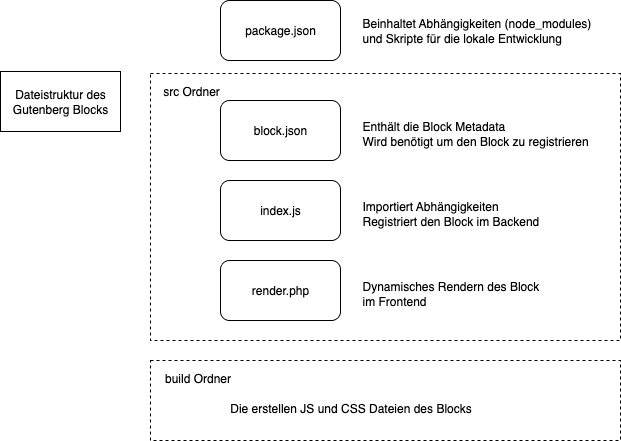
\includegraphics[width=0.88\textwidth]{gutenbergblock}
%    \caption{Gutenberg Block Struktur}
%    \label{fig:gutenberg-block-struktur}
%\end{figure}

Wenn ein Block entwickelt wird, ist es angeraten diesen als \gls{Plugin} und nicht innerhalb des Themes zu registrieren.
Dies hat den Vorteil, dass der erstellte Block unabhängig vom verwendeten Theme genutzt werden kann.
\subsection{Schlüsselkonzepte im Block Editor}
\textbf{Kombinierbarkeit}

Blöcke sind darauf ausgelegt, auf vielfältige Weise miteinander kombiniert zu werden.
Sie folgen einem hierarchischen Aufbau, bei dem ein Block in einen anderen eingebettet werden kann.
Verschachtelte Blöcke und ihr umschließender Block werden auch als Kinder und Eltern bezeichnet.
Ein Spalten-Block kann beispielsweise als übergeordneter Block fungieren und mehrere untergeordnete Blöcke in seinen einzelnen Spalten enthalten.
Die Programmierschnittstelle, die die Verwendung von Unter-Blöcken regelt, wird InnerBlocks bezeichnet~\cite{wordpress2024combination}.
\\\\
\textbf{Daten und Attribute}

Blöcke verstehen Inhalte als Attribute.
Ein Block kann eine beliebige Anzahl von Attributen beinhalten und diese werden in einer Key Value Relation definiert.
Der Key spiegelt den Namen wider und der Value ist der Wert.
Diese Inhalte sind serialisierbar in \gls{html} und werden im Block HTML (vgl. Abbildung~\ref{fig:wp-block-example}) gespeichert und so auch in der Datenbank als post\_content abgelegt.
\begin{figure}[H]
    \centering
    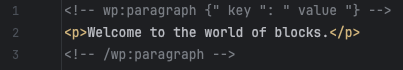
\includegraphics[width=0.6\textwidth]{wp_block_example}
    \caption{Dateistruktur eines WordPress-Blocks (eigene Darstellung)}
    \label{fig:wp-block-example}
\end{figure}

Blöcke lassen sich in zwei Kategorien unterteilen: statisch und dynamisch.
Statische Blöcke bestehen aus bereits gerenderten Inhalten sowie einem Attribut-Objekt, das bei Änderungen für das erneute Rendern verwendet wird.
Dynamische Blöcke hingegen benötigen serverseitige Daten und werden erst während der Inhaltsgenerierung gerendert~\cite{wordpress2024dataflow}.




\\\\
\textbf{Blockmuster}

Ein Blockermuster oder auch Pattern ist eine Gruppe von Blöcken, die zu einem Designmuster zusammengefasst werden.
Solche Designmuster bieten für die schnellere Erstellung komplexer Seiten einen Ausgangspunkt.
Die Größe des Blockmusters ist variabel und kann von einem einzelnen Block bis hin zu einer gesamten Seite reichen.
Themes können Designmuster registrieren, um Benutzern schnelle Startpunkte für das Verwenden von Blöcken zu bieten~\cite{wordpress2024blockpattern}.

\\\\
\textbf{Block Themes}

Anders als der Beitragseditor konzentrieren sich die Block Themes auf die Deklaration und das Bearbeiten der gesamten Website.
Hier können unter Zuhilfenahme von Blöcken die Kopf- bis hin zur Fußzeile Inhalte angepasst werden.
Die Block Themes selbst werden unterteilt in Vorlagen, die die gesamte Seite beschreiben oder Vorlagenteile, die wiederverwendbare Bereiche sein können.
Angepasste Blockvorlagen umfassen statische als auch dynamische Seiten, wie Archive, Singular, Home, 404 usw. \cite{wordpress2024EditorTemplates}


\section{Gamification im Kontext digitaler Anwendungen}

Deterding et al. definieren Gamification als \grqq{}the use of game design elements in non-game contexts\grqq{}. \cite{deterding2011gamification}
Diese Definition erfasst ein Phänomen, das in seiner Grundform nicht neu ist.
Leistungsbezogene Vergütungssysteme, Rankings und spielerische Wettkämpfe existieren in Fabriken, dem Vertrieb und Bildungseinrichtungen bereits seit Jahrzehnten. \cite{bpb2023gamification}
Die Digitalisierung hat seit etwa 2010 eine weitreichende Transformation des Gamification-Konzepts eingeleitet.
Durch die Verbreitung von Smartphones und insbesondere Wearables wie Smartwatches und Fitnessbändern haben sich neue Dimensionen der spielerischen Motivationsgestaltung eröffnet. \cite{sailer2016gamification}
Diese Entwicklung stellt einen Wechsel in der Gestaltung des Mensch-Computer-Interaktionen Paradigma dar.

Gamification hat sich von simplen Belohnungssystemen zu einem komplexen Gesamtkonzept entwickelt, das die Wahl spezifischer Elemente und Mechaniken, die Berücksichtigung des Anwendungskontextes, der Zielgruppe sowie der zu erreichenden Ziele umfasst. \cite{bpb2023gamification}
\\\\
\textbf{Abgrenzung von Serious Games}

Im Projektkontext von Charigame ist eine klare Abgrenzung zwischen Gamification und Serious Games erforderlich.
Während Serious Games als eigenständige Spiele konzipiert werden, die primär pädagogische oder Lernziele verfolgen, versteht sich die Gamification-Implementierung in Charigame als funktionale Ergänzung.
Ziel des gamifizierten Parts ist es, die Nutzerbeteiligung zu steigern und nicht als Wissensvermittlung zu dienen.
\\
Charigame verbindet somit die konventionelle Spendenaktion durch die Integration spielmechanischer Elemente, ohne dabei den ursprünglichen Zweck der Aktion zu verändern.
Der User Experience-orientierte Ansatz zielt darauf ab, die Customer Journey zu optimieren und die emotionale Bindung der Nutzer zur Spendenaktion zu erhöhen.
Dieser spielerische Ansatz dient als Mittel zur Aktivierung und nicht als Selbstzweck.
\\\\
\textbf{Strategische Bedeutung von Gamification für Spendenaktionen}

Die Integration von Gamification in Spendenaktionen adressiert mehrere strukturelle Herausforderungen traditioneller Fundraising-Ansätze.
Spendenaufrufe leiden häufig unter geringer Nutzerengagement und mangelnder Transparenz bezüglich der Verwendung der Mittel.
Gamification-Elemente schaffen hier Abhilfe durch die Visualisierung des sozialen Impacts und erhöhte Nutzerbeteiligung~\cite{golrang2021applying}.
\\\\
Die Integration spielerischer Elemente steigert sowohl die Aufmerksamkeit als auch die Reichweite sozialer Kampagnen.
Parallel dazu ermöglicht dieser Ansatz eine authentische Kommunikation des Markenimages.
Das Unternehmen kann dadurch ihre gesellschaftliche Verantwortung auf eine partizipative Weise demonstrieren~\cite{golrang2021applying}.
%TODO: QUELLE MELLE
\\\\
\section{Überblick über Coperate Social Responsibility und Charity-Plattformen}
\gls{csr} (CSR) hat sich von einem optionalen Unternehmensengagement zu einer Strategie moderner Unternehmensmaßnahmen entwickelt.
Die Europäische Kommission definiert CSR als die Verantwortung von Unternehmen für ihre Auswirkungen auf die Gesellschaft.
Hier wird ein Konzept beschrieben, das weit über die Einhaltung gesetzlicher Bestimmungen hinausgeht~\cite{european_commission2011csr}.
Diese gesellschaftliche Erwartungshaltung spiegelt sich in der zunehmenden Nachfrage nach transparenten und messbaren CSR-Maßnahmen wider, die von Verbrauchern eingefordert werden.
Wie aus der Studie der Bertelsmann-Stiftung zur gesellschaftlichen Verantwortung von Unternehmen hervorgeht, identifizieren 60\% der befragten Unternehmen die Erwartungen der Kunden als einen der wichtigsten äußeren Faktoren für ihr gesellschaftliches Engagement~\cite{bertelsmann2006gesellschaftliche}.

Die Verbindung von CSR-Maßnahmen mit digitalen, interaktiven Ansätzen stellt eine potenzielle Antwort auf diese gestiegenen Erwartungen dar.
Eine gamifizierte Charity-Plattform ermöglichen es dabei, Transparenzanforderungen zu erfüllen als auch das häufig geringe Engagement bei konventionellen Spendenaktionen zu erhöhen.
\\\\
\textbf{Charity-Plattformen}

Parallel zu dieser Entwicklung hat die Digitalisierung neue Möglichkeiten für die Umsetzung und Kommunikation von CSR-Initiativen eröffnet.
Online-Charity-Plattformen ermöglichen es Unternehmen ihre gesellschaftliche Verantwortung digital abzubilden und dabei gleichzeitig die Reichweite zu erhöhen.
Diese digitalen Plattformen fungieren als Vermittler zwischen Unternehmen, gemeinnützigen Organisationen und der Öffentlichkeit~\cite{csr40_2020}.
\\\\
\textbf{Gamifizierte Charity-Plattformen}

Die Kombination von CSR-Maßnahmen mit spielerischen Inhalten eröffnet Unternehmen neue Möglichkeiten, gesellschaftliches Engagement sichtbar und interaktiv zu gestalten.
Gamification wirkt hier als Verbindungsstück, das das in CSR-Anwendungen häufig geringe Nutzerengagement adressiert und erhöht.
Charity-Plattformen, die auf Gamification-Elemente setzen, verbinden damit zwei wesentliche Aspekte.
Die wachsende Erwartungshaltung an transparente CSR-Initiativen und den Trend zu interaktiven, nutzerzentrierten digitalen Anwendungen.
Damit ist der theoretische Rahmen gesetzt, innerhalb dessen das Projekt \textit{Charigame} verortet werden kann.
Im folgenden Kapitel wird der Projektkontext dargestellt, um die praktische Umsetzung und Weiterentwicklung der \gls{Plugin}-Architektur nachvollziehbar zu machen.